In this chapter we describe a software framework called Rheos, which demonstrates an approach for reasoning about large genomic datasets utilizing concepts of service-orientation and data streaming in contrast with traditional genomic data analysis frameworks\autocite{depristo2011framework} that take a procedural batch-based approach. Rheos' focus on service-orientation and streaming allow the users to make active tradeoff decisions between analysis time, cost, and quality as well as setting up precise operational Service Level Agreements, both between Rheos components, and between Rheos and external systems, as we describe in detail below.

\section{General Framework Design}

As already discussed in Chapters \ref{ch:introduction} and \ref{ch:background}, the general problem consists of collecting DNA samples from a population of individuals under study, sequencing these samples using Next Generation Sequencing techniques, identifying the mutations that are present, annotating their functional impact and utilizing the obtained data in a downstream data analysis with research or clinical decision-making goals. While there is a great variety of possible downstream analyses that may be performed depending on the individual goals of the analyst, there is a fairly well established set of steps for processing of the raw NGS data into a set of annotated variants, and it is these steps that we target with this work. The typical approach that is in widespread use today is to collect a batch of samples and then process each sample individually with a sequence of individual tools, that may be described via a higher-level workflow construct (such as in Figure \ref{fig:gatk_best_practices}, or using a framework like Butler, as described in Chapters \ref{ch:butler_architecture}, \ref{ch:butler_implementation}). There are, however, a number of factors that leave room for improvement in this model. These improvements lie along a set of dimensions that we describe briefly in the Introduction via a utility function $U_i = C_i + T_i + A_i$ for sample $i \in [1,N_s]$  that needs to be optimized, and that we describe in more detail here.

We use the following definitions throughout the text:

\begin{table}[!ht]
    \caption{Rheos common definitions}
    \label{tab:rheos_notation}
    {\begin{tabular}{lp{7cm}}
    \toprule
    Symbol & Description \\
    \midrule
    $N_p$ & Number of people \\
    $P = \{p_i : i \in [1,N_p]\}$ & Set of individuals under study \\
    $N_s$ & Number of samples \\
    $S = \{s_i : i \in [1,N_s]\}$ & Set of sequenced DNA samples. Each individual can have one or more samples. \\
    $A_i $ & Accuracy score of analysis for sample $i$ (precise definition of Accuracy TBD) \\
    $C_i = c_{g_i} + c_{s_i} + c_{a_i} + c_{r_i}$ & Cost score of data generation, storage, analysis, and retrieval respectively \\
    $T_i$ & Time score to process sample $i$ \\
    $U_i = C_i + T_i + A_i$ & A utility function for individual $i$ that penalizes high cost, high processing time, and low accuracy\\
    $U = \sum_{i=1}^{N_s} U_i$ & Overall utility of processing $N_s$ samples through Rheos.\\
    \bottomrule
    \end{tabular}}
\end{table}


\section{Data Streaming Architecture}

The overall technical architecture of the Rheos system is set up as a Service Oriented Architecture (SOA)\autocite{shaw1996software} which is an information system architecture paradigm where the overall problem that the system is trying to solve is broken down into a collection of loosely-coupled components called services. Each service has a well defined interface of inputs that it accepts and outputs that it produces. Services can be combined and orchestrated together to produce the overall desired output for the system. A key distinguishing feature of this architectural approach is that each service can be individually optimized to fulfill its contract most efficiently helping break down some of the performance limitations brought about by the necessity to simultaneously tackle competing constraints in more monolithic information system designs. Additionally, within a services framework, the dependencies between separate services can be negotiated not only in terms of service interfaces, but also in terms Service Level Agreements which constitute Quality of Service promises made by one service to its dependents\autocite{ingham2000constructing}. Because it is unlikely that a service designer will be able to accurately foresee all of the demands that will be placed on a service during its lifetime the SLAs provide a valuable feedback framework through which the service can be evaluated as it operates in production, as well as serving as a basis for negotiating evolving requirements between dependent services.

While general web services can support any data processing paradigm, in the Rheos framework we adopt a data streaming approach\autocite{babcock2002models}. In this approach we assume that the input to any service is a randomly ordered sequence of messages $M = {m_1, m_2, ....}$ where each message represents a fact about the underlying domain that the service reasons over, as well as some metadata, including an identifier, and a variety of timestamps of interest. The content of each message may provide a datum, such as the measurement of a quantity of interest, or signal that a particular event has taken place. It is in general assumed that the data stream is infinite in size, that messages may arrive out of order, and that any message that is placed in the stream is observed at most once, and may, in fact, never be observed. Messages are typically not sent directly from one service to another, instead the transfer of messages is mediated by a queuing system using a publish-subscribe\autocite{eugster2003many} model. Under this model each queue acts as a \emph{topic}. Message producers can publish data to the topic, and message consumers subscribe to receive messages from the topic. A message is consumed from the queue only after all of the subscribed consumers have seen it. End users retrieve information from the system via a set of User Interfaces that support both push (notifications) and pull (querying) models of data retrieval. A more detailed description of the architectural aspects of the system follows:

\subsection{Service-Oriented Data Streaming Model}

A data stream $M_{s,d} = {m_1, m_2, ....}$ is a sequence of datagrams transmitted over the network with the following properties:

\begin{itemize}
    \item The stream has a source $s$ and a destination $d$.
    \item A message $m$ in the stream is a tuple of the form $(header, payload)$, where:
    \begin{itemize}
        \item $header$ is a tuple of the form $(id, \dots)$ that holds at minimum a unique identifier $id$ for messages, and may hold additional metadata.
        \item $payload$ is an arbitrary data structure that holds the informational content of the message. 
    \end{itemize}
    \item $|M| = \infty$ by assumption.
    \item Messages may not arrive at destination $d$ in the same order that they were sent from source $s$.
    \item If $t_{i,s}$ is the time message $m_i$ leaves the source $s$ and $t_{i,d}$ is the time of arrival at destination $d$, then $\sup_i \{t_{i,d} - t_{i,s}\} = \infty$, i.e. a given sent message may never arrive at its destination.
\end{itemize}

A service $S = \{o_i\}$ is a collection of operations $o_i$ that act on one or more input data streams $\{M_i\}$ to produce one or more transformed output data streams $\{M_j\}$. Specifically:

An operation $O$ is a tuple of the form  $O = (i,o,p,f)$, where:
\begin{itemize} 
    \item $i = \{M_j, j \in [0, K]\}$ is a set of $K \ge 0$ input data streams.
    \item $o = \{M'_j, j \in [0, L]\}$ is a set of $L \ge 0$ output data streams.
    \item $f:M^K \mapsto M'^L$ is a transformation function that produces messages $m'$ in the output streams based on messages $m$ observed in the input streams.
    \item $p = \{p_i\}$ is a set of potentially optional query parameters.  
\end{itemize}

There are several distinct categories of operations that a service can perform on a set of input streams. We describe these here:

\paragraph{Windowing Function} - Service $S$ observes a sliding window, which is a sample of size $n$ of messages from stream $M_i$ and computes a summary statistic (see Figure \ref{fig:stream_window_function}) over the sample which is meant to be an approximation of the corresponding population parameter.

\begin{figure}[H]
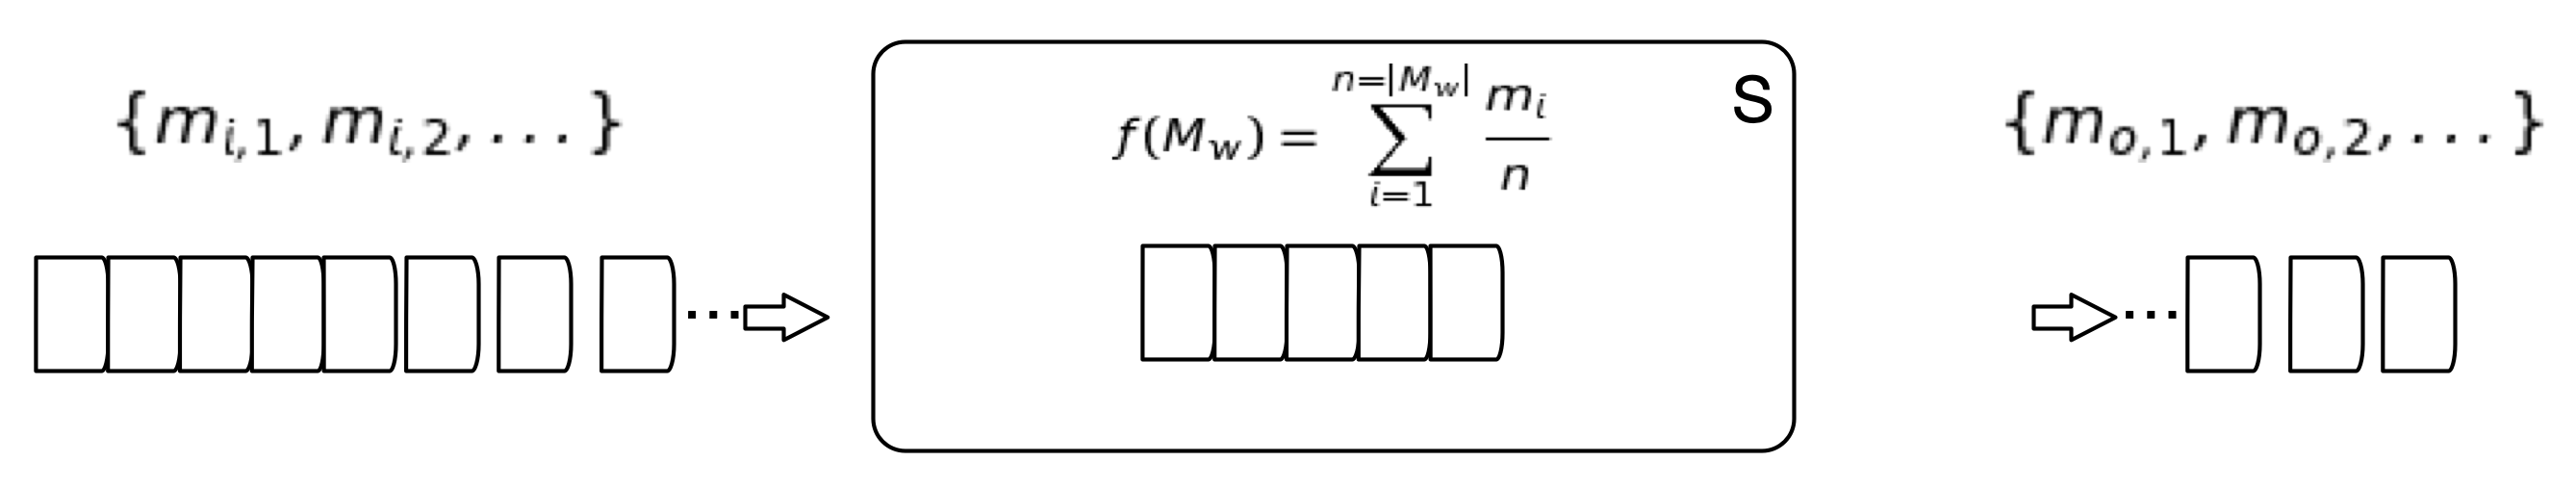
\includegraphics[scale=0.6]{stream_window_function}
\centering
\caption {Service S computes a summary statistic over a window of messages from stream $M$}
\label{fig:stream_window_function}
\end{figure}
 
\paragraph{Decorator Function} - Service $S$ observes messages $m_i$ and applies a function that augments (decorates) each message with additional attributes (see Figure \ref{fig:stream_decorator_function}) producing augmented messages $m_o$ as output.

\begin{figure}[H]
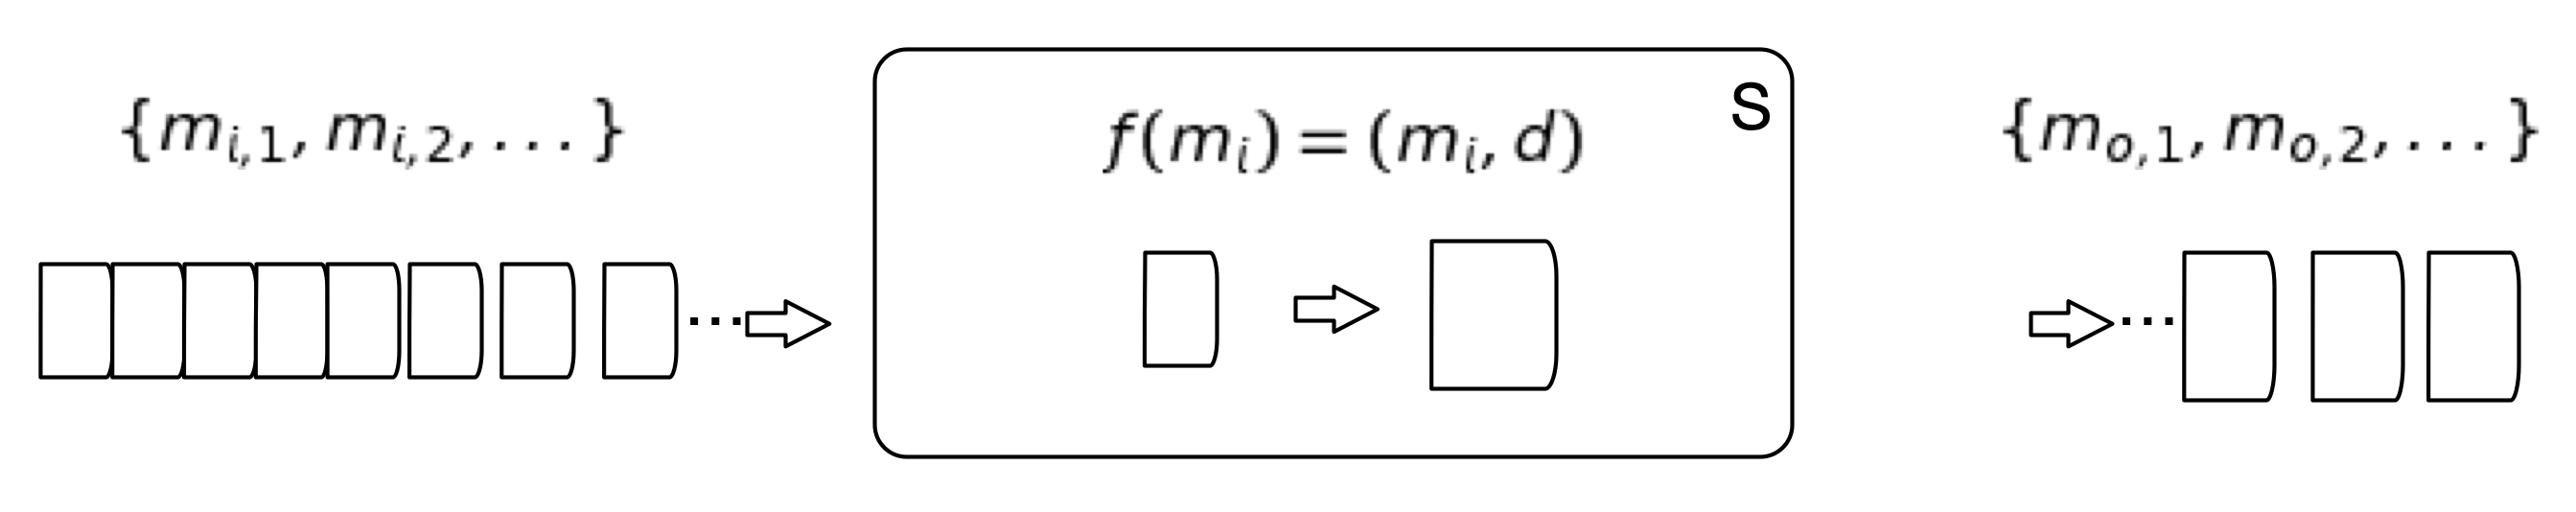
\includegraphics[scale=0.6]{stream_decorator_function}
\centering
\caption {Service S computes a summary statistic over a window of messages from stream $M$}
\label{fig:stream_decorator_function}
\end{figure}

\paragraph{Filter Function} - Service $S$ observes messages $m_i$ and applies a function $f:M\mapsto\{True,False\}$ that evaluates to a boolean value (see Figure \ref{fig:stream_decorator_function}). Only messages that map to $True$ are emitted as output.

\begin{figure}[H]
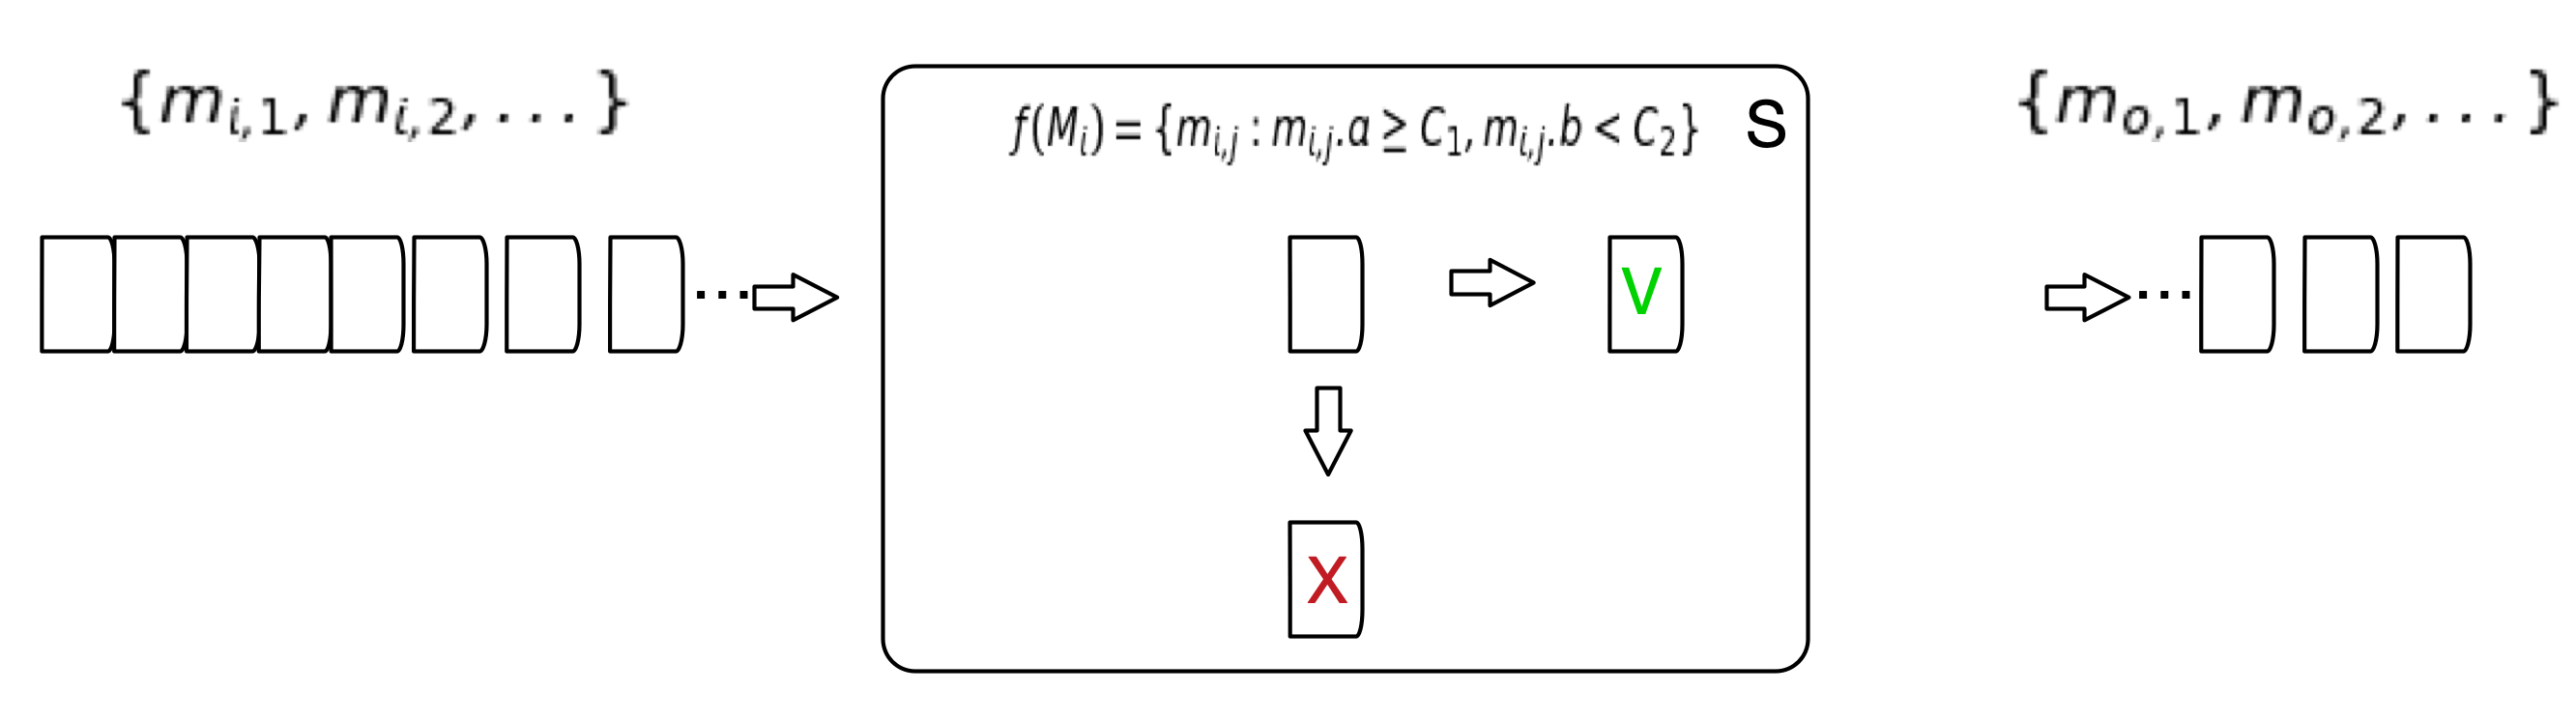
\includegraphics[scale=0.6]{stream_filter_function}
\centering
\caption {Service S filters messages from input stream $M$ and only allows through those that pass the filtering condition.}
\label{fig:stream_filter_function}
\end{figure}

\paragraph{Aggregator Function} - Service $S$ observes messages $m_i$ and applies a function $f:M\mapsto\{True,False\}$ that evaluates to a boolean value (see Figure \ref{fig:stream_decorator_function}). Only messages that map to $True$ are emitted as output.

\begin{figure}[H]
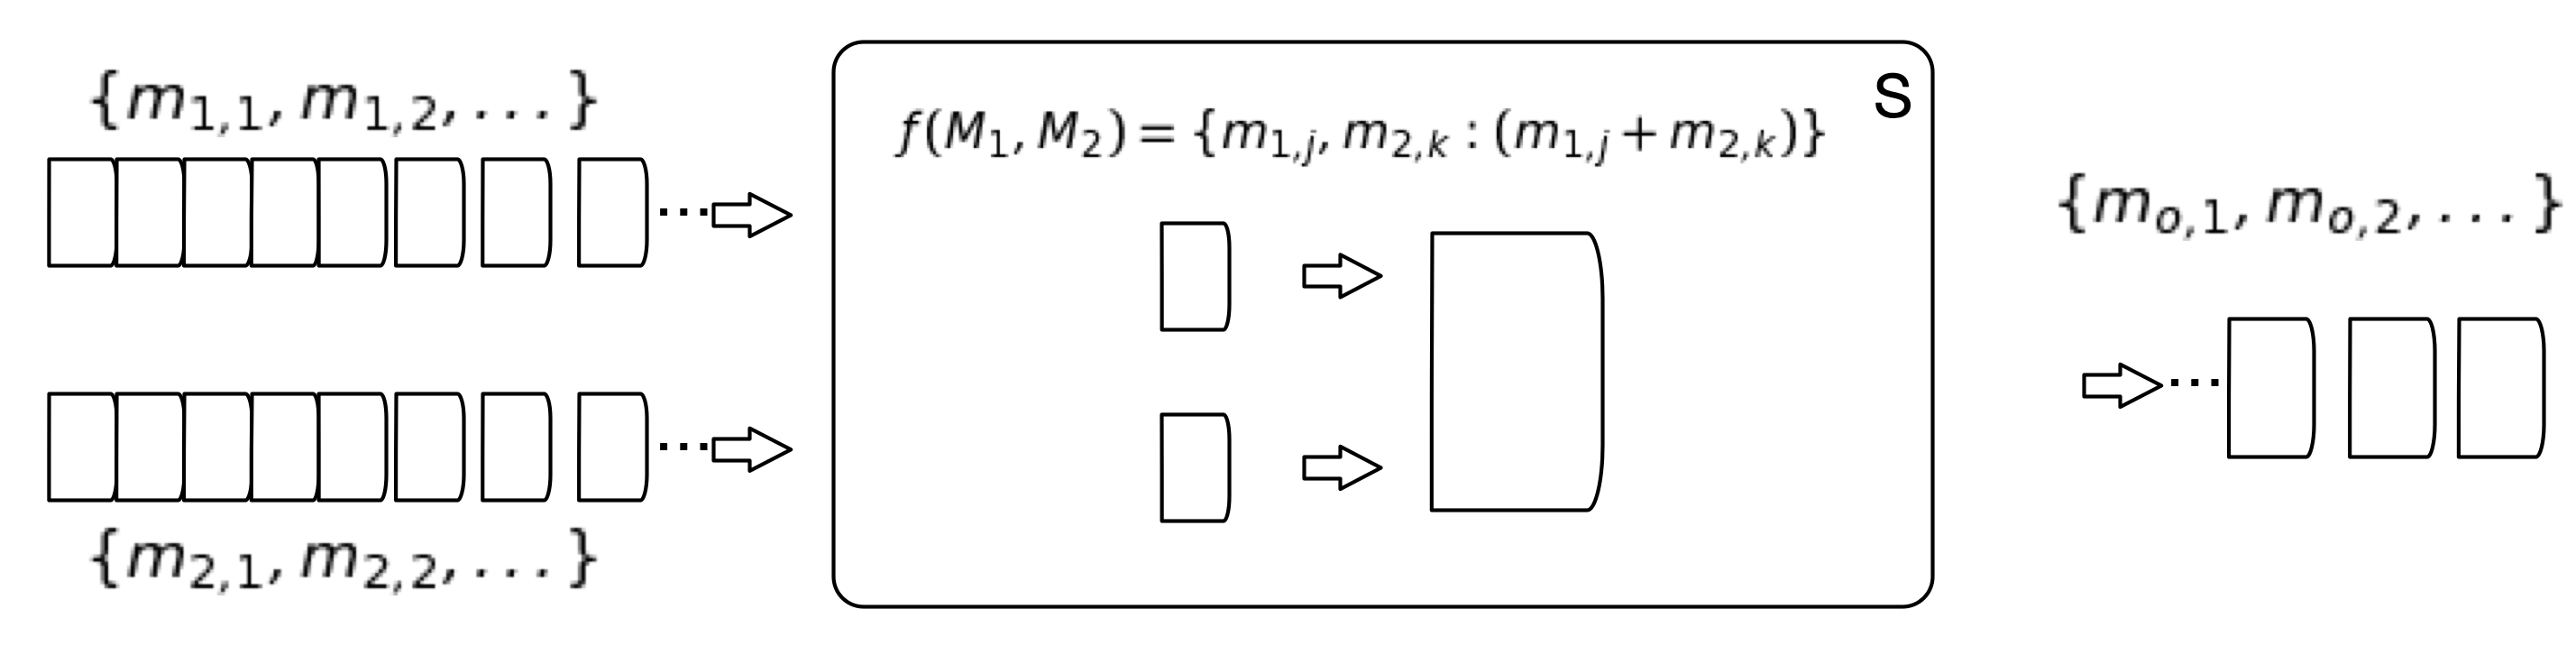
\includegraphics[scale=0.6]{stream_aggregator_function}
\centering
\caption {Service S filters messages from input stream $M$ and only allows through those that pass the filtering condition.}
\label{fig:stream_aggregator_function}
\end{figure}


\paragraph{Local State Aggregator Function} - Service $S$ observes messages $m_i$ and applies a function $f:M\mapsto\{True,False\}$ that evaluates to a boolean value (see Figure \ref{fig:stream_decorator_function}). Only messages that map to $True$ are emitted as output.

\begin{figure}[H]
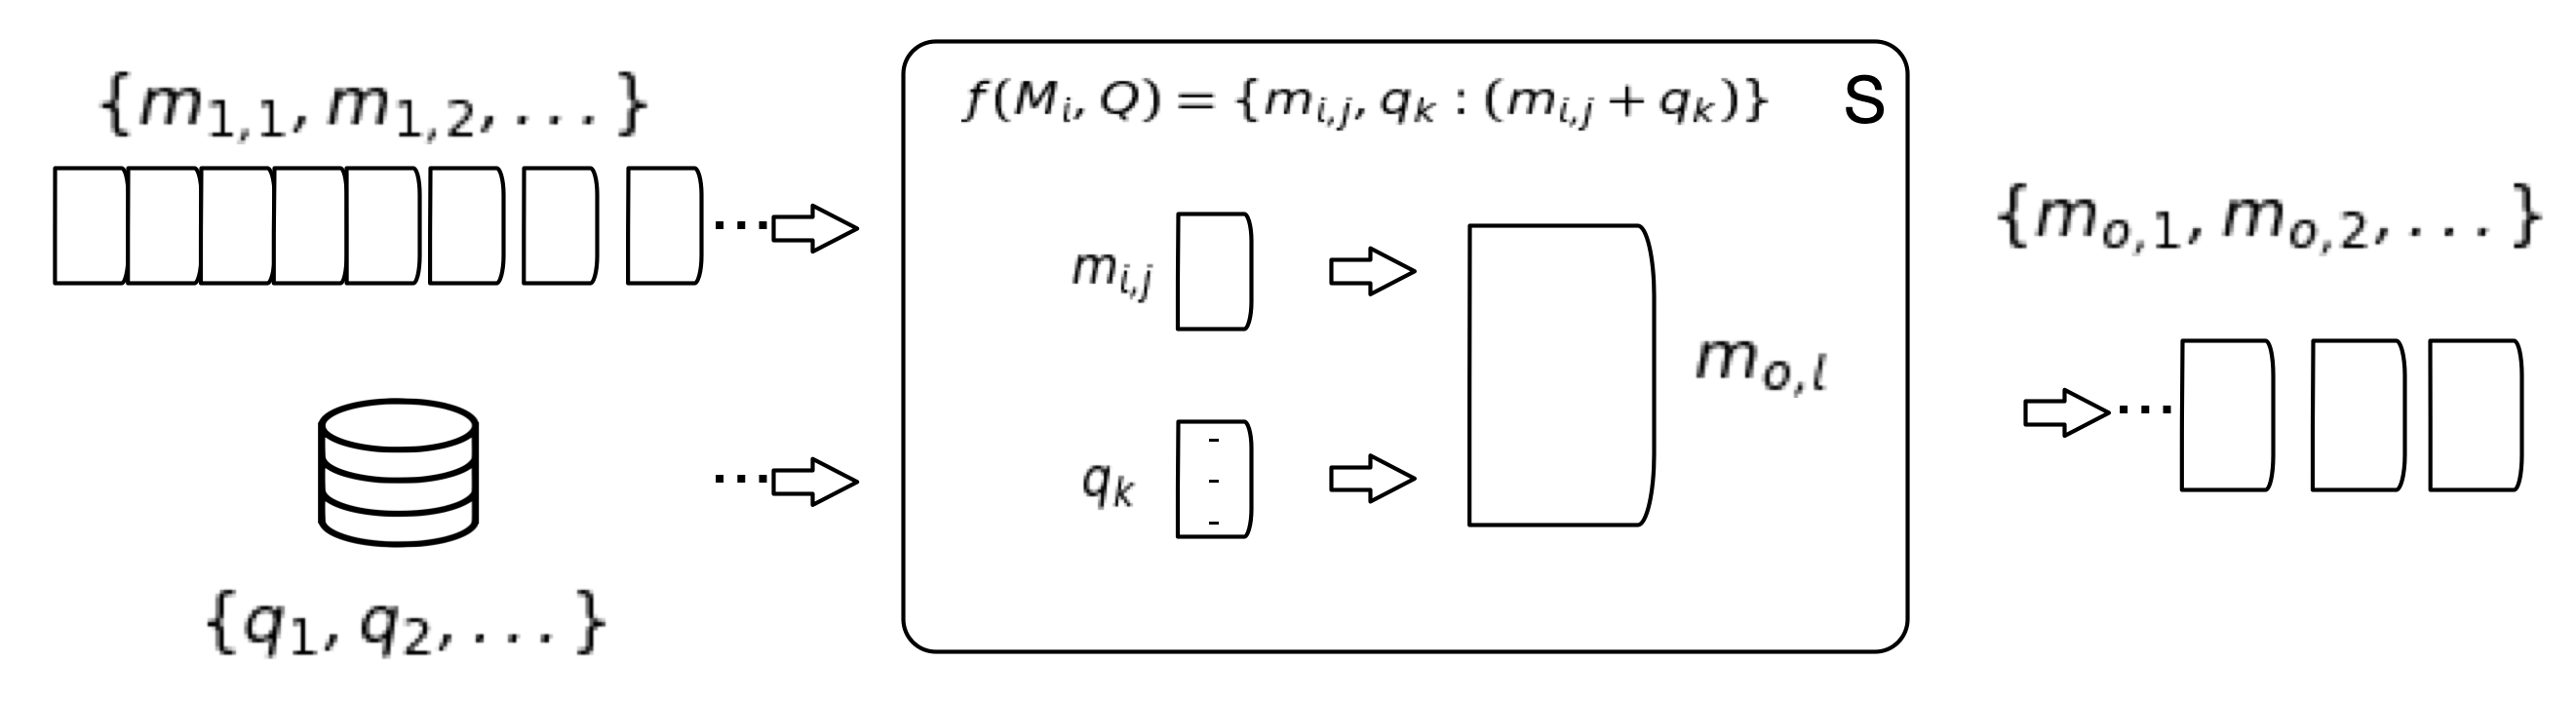
\includegraphics[scale=0.6]{stream_local_state_aggregator_function}
\centering
\caption {Service S filters messages from input stream $M$ and only allows through those that pass the filtering condition.}
\label{fig:stream_local_state_aggregator_function}
\end{figure}


\paragraph{Persistence Function} - Service $S$ observes messages $m_i$ and applies a function $f:M\mapsto\{True,False\}$ that evaluates to a boolean value (see Figure \ref{fig:stream_decorator_function}). Only messages that map to $True$ are emitted as output.

\begin{figure}[H]
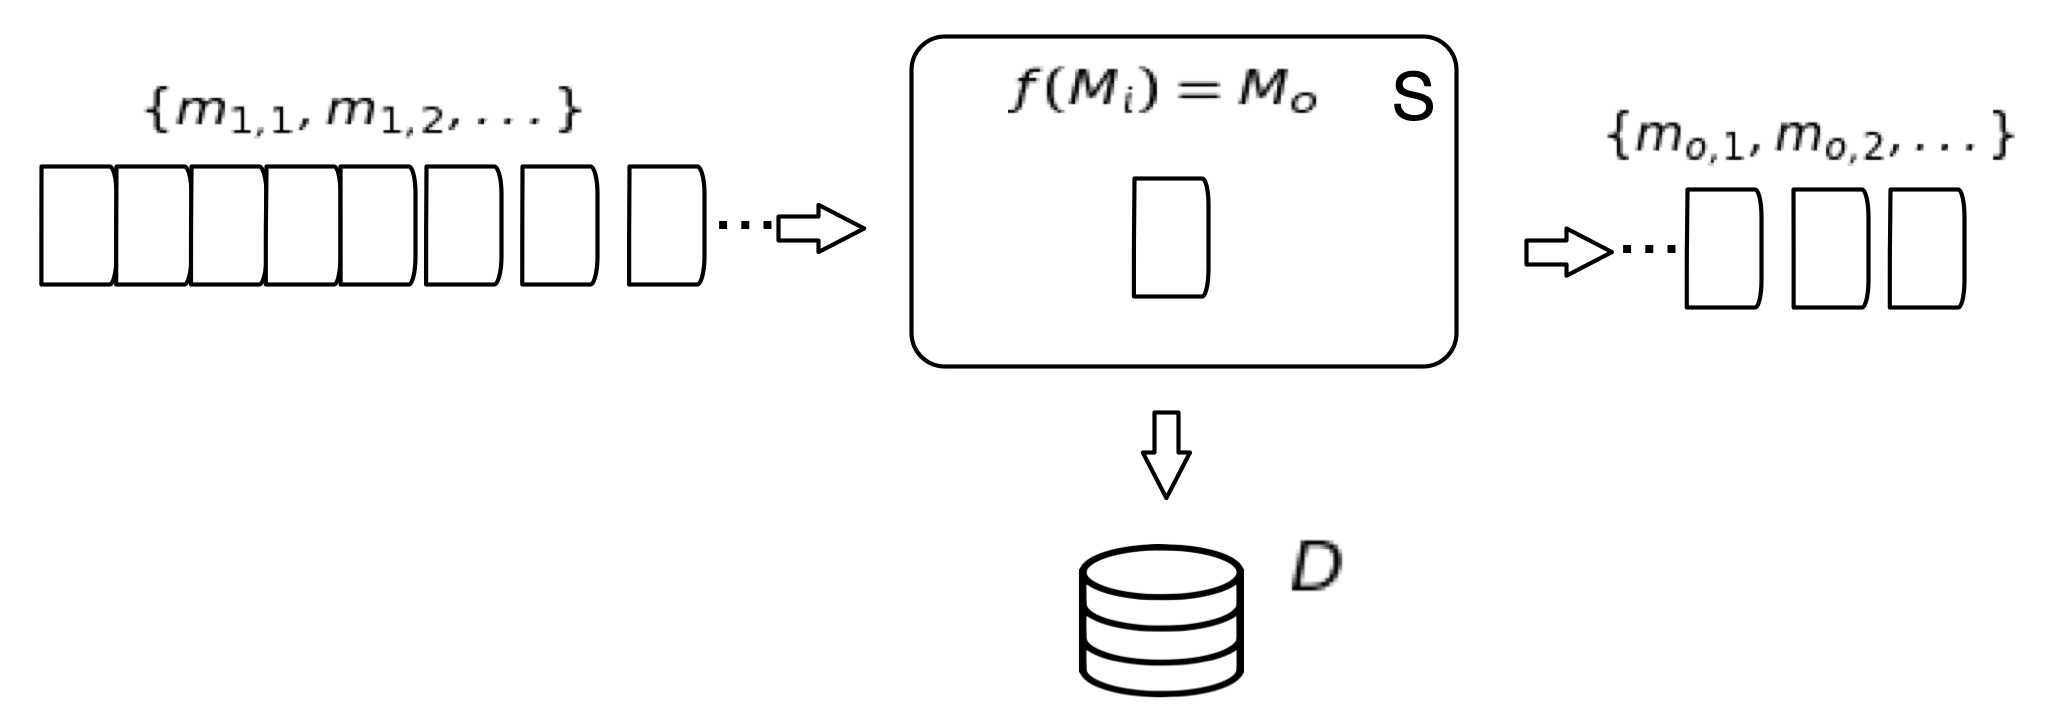
\includegraphics[scale=0.6]{stream_persistence_function}
\centering
\caption {Service S filters messages from input stream $M$ and only allows through those that pass the filtering condition.}
\label{fig:stream_persistence_function}
\end{figure}

\paragraph{Query Function} - Service $S$ observes messages $m_i$ and applies a function $f:M\mapsto\{True,False\}$ that evaluates to a boolean value (see Figure \ref{fig:stream_decorator_function}). Only messages that map to $True$ are emitted as output.

\begin{figure}[H]
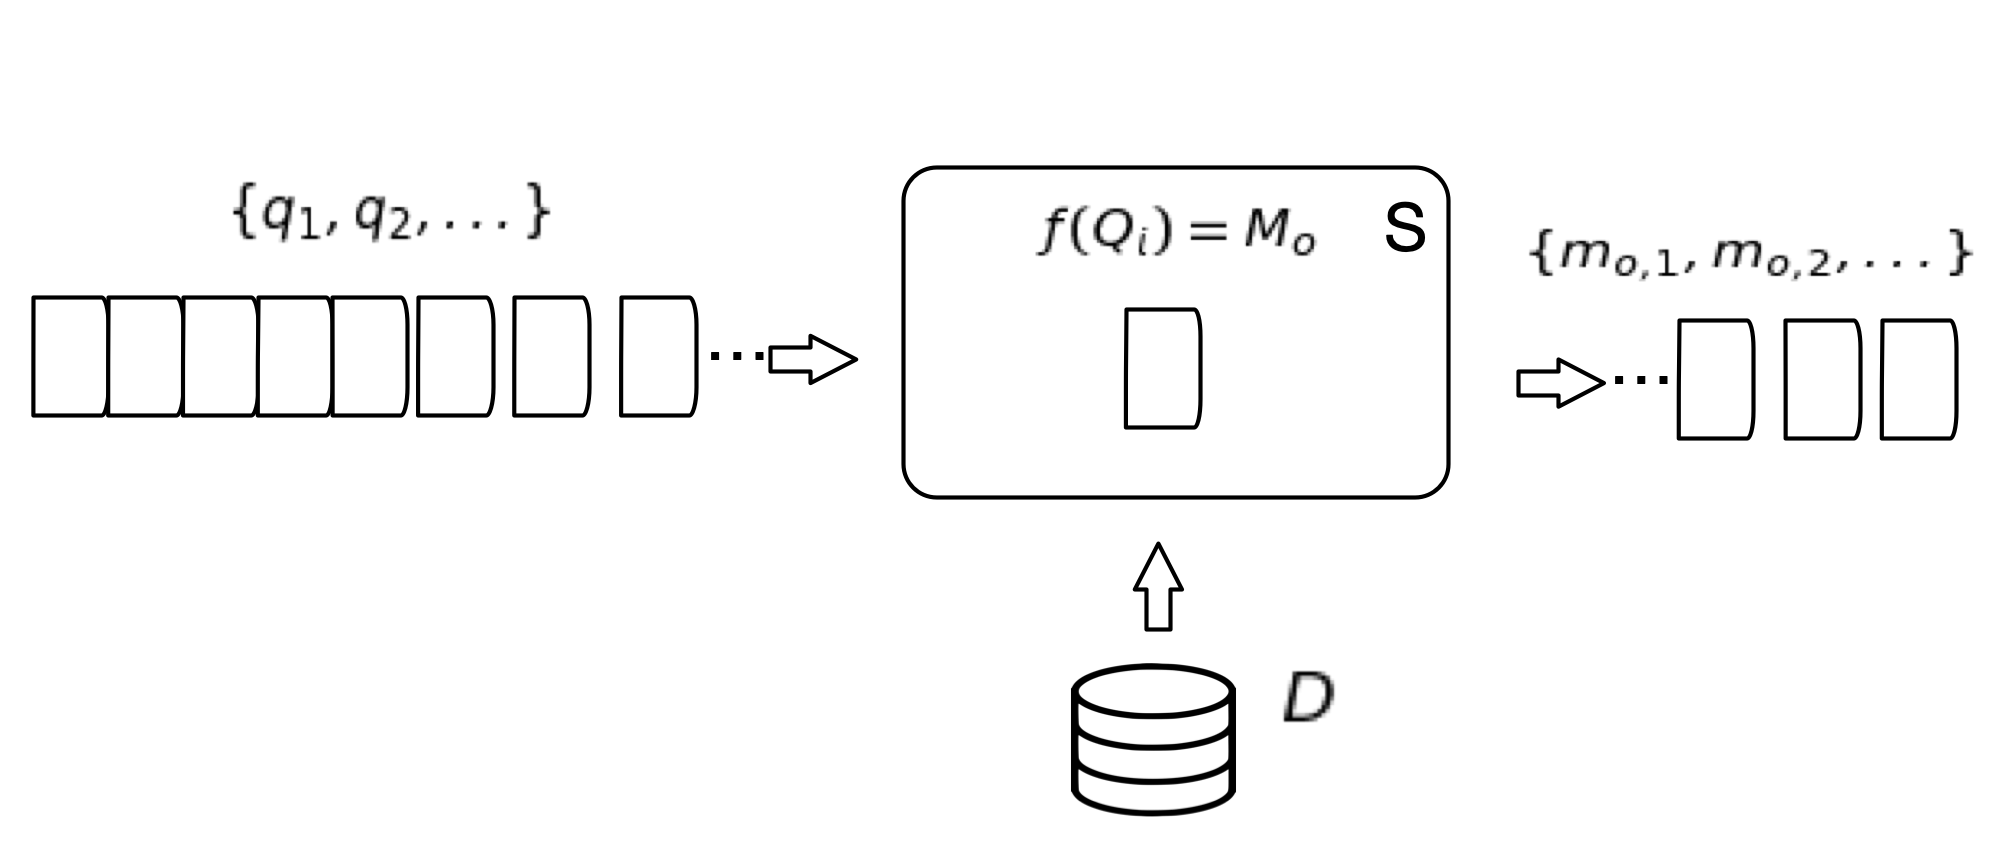
\includegraphics[scale=0.6]{stream_query_function}
\centering
\caption {Service S filters messages from input stream $M$ and only allows through those that pass the filtering condition.}
\label{fig:stream_query_function}
\end{figure}


Aggregator
Local State Aggregator
Persistence
Query


    

-----------------
Set up the general architecture of information flow through the system - types of entities, communication channels, contracts, SLAs, capabilities:

\begin{itemize}
 \item Each stream is a collection of randomly ordered datagrams.
 \item A datagram may constitute data or an event.
 \item The rate of the stream is understood.
 \item A service applies a transformation to the stream by virtue of making a decision upon inspecting stream contents.
 \item A service makes decisions based on:
 \begin{itemize}
    \item Individual datagrams
    \item Sliding windows of datagrams
    \item Particular sequences of datagrams
    \item Integration of incoming stream signal with a static data store
    \item Combinations of multiple streams
 \end{itemize}
 \item A service emits a new stream as output.
 \item A service may decorate an existing stream with new info or create new datagrams.
 \item A service may persist data to a permanent store.
 \item The rate at which the service can make decisions is understood (along with limiting conditions).
 \item Communication between services is mediated via queues.
 \item Services provide an SLA on uptime, latency, throughput, etc.
 \item Services fail fast.
 \item System output supports push and pull modes.
\end{itemize}
\section{Domain-specific Problems}

Describe specific problems that need to be addressed by the system in a stream-based formulation - how to go from a collection of raw reads to a set of annotated variants: map reads, perform QC filtering, model loci, assemble alternative haplotypes, call variants, filter variants, annotate, produce output.  


\begin{itemize}
    \item Perform read QC
    \item Align reads to reference
    \item Collect read stream statistics
    \item Assemble local read contigs
    \item Model individual loci
    \item Call variants (maybe need to split by variant types)
    \item Genotype variants
    \item Filter variants
    \item Annotate variants
    \item Output variants
\end{itemize}


\section{Services of Rheos}

Provide a mapping from the domain-specific problems onto a particular implementation in the data streaming architecture. List services, their responsibilities, contracts, etc.

\begin{description}
    \item [Metadata] - Take in metadata related to patients, samples, files, etc. In: Metdata records, Out: ingestion confirmation events.
    \item [Read Streaming] - Take data from outside the system (file, web service, etc) and turn it into a standard stream. In: files, external streams, Out: internal read stream.
    \item [Read Persistence] - Store reads on disk, index. In: read stream, Out: persistence confirmation events.
    \item [Read Statistics] - Look at read stream and calculate various approximate stats of interest - insert size, GC-bias,  etc. In: read stream, Out: running stats of interest
    \item [QC] - Compute QC score for reads. In: reads, Out: reads with QC score
    \item [Read Filtering] - Filter out low quality reads based on configured parameters. In: reads with QC score, Out: filtered reads.
    \item [Read Mapping] - Align reads to reference genome. In: stream of reads, Out: streams of mapped, unmapped, split reads.
    \item [Local Assembly] - Local assembly of reads into candidate haplotypes. In: stream of aligned reads, Out: Updated haplotypes event.
    \item [Haplotype Persistence] - Storage and lookup of candidate haplotypes. In: stream of reads, Out: persistence confirmation events, stream of haplotypes.
    \item [Variant Calling] - Evaluate candidate haplotypes for presence of variation. In: haplotype update events, Out: variant update events.
    \item [Variant Persistence] - Storage and lookup of variants. In: stream of reads, Out: persistence confirmation events, stream of variants.
    \item [Genotyping] - Genotype variant sites. In: variant update stream, Out: genotype update events.
    \item [Variant Filtering] - Filter out low quality variants. In: stream of variants, Out: filtered stream of variants.
    \item [Variant annotation] - Annotate variants for functional impact. In: stream of variants, Out: stream of annotated variants.
    \item [Output variants] - Format variants for external output. In: stream of variants, Out: files, external variant stream.
    \item [Notification] - Notify the user when events of interest occur. In: any stream, Out: stream of notifications.
\end{description}

\section{Proof of concept implementation}

Describe actual implementation efforts. Focus on very basic use case (take already mapped reads from a file, turn them into a stream, use stream to call SNPs, maybe some Indels/SVs). Demonstrate some comparison metrics compared to other callers. Demonstrate some service-level metrics (throughput etc.)

\section{Conclusions}
Rheos is great!